%%
%% Copyright 2007, 2008, 2009 Elsevier Ltd
%%
%% This file is part of the 'Elsarticle Bundle'.
%% ---------------------------------------------
%%
%% It may be distributed under the conditions of the LaTeX Project Public
%% License, either version 1.2 of this license or (at your option) any
%% later version.  The latest version of this license is in
%%    http://www.latex-project.org/lppl.txt
%% and version 1.2 or later is part of all distributions of LaTeX
%% version 1999/12/01 or later.
%%
%% The list of all files belonging to the 'Elsarticle Bundle' is
%% given in the file `manifest.txt'.
%%

%% Template article for Elsevier's document class `elsarticle'
%% with numbered style bibliographic references
%% SP 2008/03/01
%%
%%
%%
%% $Id: elsarticle-template-num.tex 4 2009-10-24 08:22:58Z rishi $
%%
%%
\documentclass[preprint,12pt,3p]{elsarticle}

%% Use the option review to obtain double line spacing
%% \documentclass[preprint,review,12pt]{elsarticle}

%% Use the options 1p,twocolumn; 3p; 3p,twocolumn; 5p; or 5p,twocolumn
%% for a journal layout:
%% \documentclass[final,1p,times]{elsarticle}
%% \documentclass[final,1p,times,twocolumn]{elsarticle}
%% \documentclass[final,3p,times]{elsarticle}
%% \documentclass[final,3p,times,twocolumn]{elsarticle}
%% \documentclass[final,5p,times]{elsarticle}
%% \documentclass[final,5p,times,twocolumn]{elsarticle}

%% if you use PostScript figures in your article
%% use the graphics package for simple commands
%% \usepackage{graphics}
%% or use the graphicx package for more complicated commands
\usepackage{graphicx}
%% or use the epsfig package if you prefer to use the old commands
%% \usepackage{epsfig}

\usepackage{subfigure}
\usepackage[linesnumbered,ruled]{algorithm2e}

%% The amssymb package provides various useful mathematical symbols
\usepackage{amssymb}
%% The amsthm package provides extended theorem environments
%% \usepackage{amsthm}

%% The lineno packages adds line numbers. Start line numbering with
%% \begin{linenumbers}, end it with \end{linenumbers}. Or switch it on
%% for the whole article with \linenumbers after \end{frontmatter}.
%% \usepackage{lineno}

%% natbib.sty is loaded by default. However, natbib options can be
%% provided with \biboptions{...} command. Following options are
%% valid:

%%   round  -  round parentheses are used (default)
%%   square -  square brackets are used   [option]
%%   curly  -  curly braces are used      {option}
%%   angle  -  angle brackets are used    <option>
%%   semicolon  -  multiple citations separated by semi-colon
%%   colon  - same as semicolon, an earlier confusion
%%   comma  -  separated by comma
%%   numbers-  selects numerical citations
%%   super  -  numerical citations as superscripts
%%   sort   -  sorts multiple citations according to order in ref. list
%%   sort&compress   -  like sort, but also compresses numerical citations
%%   compress - compresses without sorting
%%
%% \biboptions{comma,round}

% \biboptions{}


\journal{IPL}


\begin{document}

\begin{frontmatter}


%\mainmatter  % start of an individual contribution

% first the title is needed
\title{Gradient Boosting to Precompute Multiple Evidences in Search Index Construction}

\author[mymainaddress]{Sheila Silva}
\author[mymainaddress]{Edleno Moura}
\author[mysecondaryaddress]{P{\'a}vel Calado}
\author[mymainaddress]{Altigran Silva}

\address[mymainaddress]{Universidade Federal do Amazonas, Brasil}
\address[mysecondaryaddress]{INESC-ID, Instituto Superior Técnico, Universidade de Lisboa}


\begin{abstract}

There has been an ongoing effort to apply \textit{learning to rank} techniques in search engines query processing, with the goal of enhancing the quality of the search results. Most works, however, focus on applying such techniques at query time, thus adding complexity to the search process. In this paper we address the problem of using a learning to rank technique to fuse sources of relevance evidence at indexing time. We propose to use a modified Gradient Boosted Regression Tree algorithm to generate a \textit{unified term impact} to be stored in the index. The unified term imapct is the only value needed later for ranking the documents, thus greatly reducing the effort needed to compute the document scores. Our approach achieves better results in quality, when compared to state of the art baselines, and greatly reduces the amount of time required for computing search results. In addition, we show that is possible to obtain significant gains in index compression with virtually no loss in the final quality of results. This is achieved by exploiting a simple, yet effective, reduction of size in the representation of the unified term impact values, when the inverted list is created. Our best approach was able to achieve 91\% compression rate of the index, while keeping the quality of results on par with methods that do not use compression.


\begin{keyword}
\texttt Learning to Rank \sep Search Engines \sep Indexing \sep LambdaMART \sep Gradient Boosting
\end{keyword}

\end{abstract}
\end{frontmatter}


%%
%% Start line numbering here if you want
%%
% \linenumbers

%% main text

\section{Introduction}
\label{intro}

A fundamental aspect of current Web search engines is the quality of the ordered list of results. Users expect the answers to their queries to be shown at the top of the list and rarely tend to go beyond the first page displayed~\cite{saraiva2001rank}. When unstatisfied, in the best case, users will issue new queries, thus increasing the load of the system, while in the worst case, they will simply try a competitor system. Moreover, modern search engine users are used to experience fast query processing times, regardless of the size of the dataset, and any noticeable increase in waiting time can be a fatal blow to the their perception of the quality of the system. Thus, although commercial search engines can receive tens of thousands of queries per second, each one requiring access to a massive collection of data, computational efficiency cannot be obtained at the cost of quality. 

The issue of quality is usually addressed through a class of machine learning techniques commonly known as \textit{learning to rank} (L2R). Query processing by a L2R-based search engine is performed in two steps: first, the top-k documents for a query are retrieved using simple ranking strategy, such as BM25; second, the documents are re-ranked with the more expensive L2R model.

An important aspect of modern search engines is the use of a large number of distinct sources of relevance evidence to build the L2R model. Relevance evidence can be defined as the set of features that can be extracted from the documents, which collectively make the document relevant to the query issued by the user. Examples of such sources of relevance evidence are frequencies of terms in text, urls, titles, and other parts of the document, part of speech tags, web link graph analysis, anchor text of the incoming links to a web page, HTML structure, such as titles and headings, url tokenization, among others~\cite{baezaribeiro2011modinforet}. 

These distinct sources of relevance evidence are used to compute the query result rankings. This is achieved by fusing all sources into a single document score, for each document in the final ranking. In the past few decades, most work on fusing evidence has been done with the deployment of L2R methods such as RankBoost~\cite{freund2003efficient}, Genetic Programming based methods~\cite{de2007combined, silva2009evolutionary}, RankSVM~\cite{joachims2002optimizing} and, the current state of the art, Gradient Boosting method LambdaMART~\cite{wu2010lambdamart}. These methods use examples of queries and their respective results, to train a supervised learning model that determines the relative position of the documents in the result list. Once trained, the model can be used during query processing to determine the final ranking. This approach, however, inadvertently adds computational costs to query processing, which may lead to a drop in time  performance.

\newcommand{\lepref}{LePrEF}

To mitigate this problem, an alternative approach has been proposed --- Learn to Precompute Evidence Fusion (\lepref)~\cite{costa2012lepref}, also based on supervised learning. \lepref\ proposes to implement the bulk of the evidence fusion during indexing time, generating a single inverted index containing unified entries regarding all features, called \textit{Unified Term Impacts} (UTIs). Fig.~\ref{fig:arq} shows a diagram of \lepref's architecture. Contrary to traditional systems, \lepref\ does not maintain separate inverted indexes for each source of relevance evidence. Instead, it creates a single inverted index containing the fused values for all sources, i.e. the UTIs. Each UTI is computed based on a trained L2R model and, at query time, the search engine needs only to add each of the query term's UTI to directly obtain the document scores.

\begin{figure}
\begin{center}
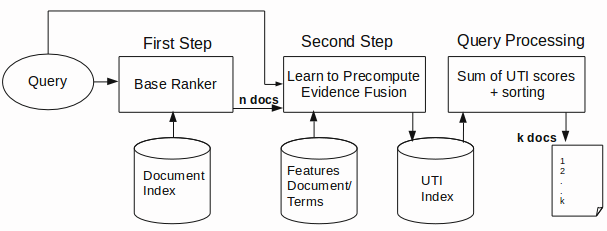
\includegraphics[width=12cm, height=5cm]{im_arquitetura.png}
\caption{The LePrEF architecture. }
\label{fig:arq}
\end{center}
\end{figure}

\newcommand{\lambdamart}{LambdaMART}

While the authors of LePrEF show that it can lead to high quality results, they're approach has several drawbacks.  First, UTIs are computed using Genetic Programming~\cite{XXXX}, an optimization method that has a high computational cost during the model training phase. Second, XXXXXX. In this work, we avoid these issues by proposing an adaptation of \lambdamart~\cite{wu2010lambdamart}, a gradient boosting algorithm, to compute the UTIs of each term at the indexing time. \lambdamart\ was designed specifically to optimize ranking quality metrics, such as NDCG, and was shown to be very effective in traditional (i.e. query-time) L2R tasks. Our adaptation allows for improvements in the quality of the rankings produced varying from XXXX through XXXX points in precison, when compared to the state of the art. Also, we are able to achieve these results in XXXX of the time required by LePref. In addition to the improvements in rank quality, we also show that a simple compression technique can be applied to the inverted index containing the UTIs, reaching gains of XXXX in space requirements, without a significant loss of quality.

The remaining  of this article is organized as follows: In Section~\ref{relatedwork}, we discuss related work and an overview of the basic concepts involved. Section ~\ref{lambda} presents the proposed method describing how we use LambdaMART to generate query term UTI scores in the indexing time. Section ~\ref{experiments} presents the experimental setup followed by experimental results in comparison to current baselines in Section~\ref{results}. Finally, Section~\ref{conclusion} presents the conclusive remarks and directions to future research.


\section{Background and Related Work}
\label{relatedwork}

Machine learning has been successfully adopted in a wide range of Information Retrieval applications, including in important components of search systems, such as query processing~\cite{de2007combined,fan2004effects,freund2003efficient,joachims2002optimizing}, crawling~\cite{Santos2015}, classifying queries according to user goals~\cite{herrera2010exploring}, and indexing~\cite{costa2012lepref}. Here, we will focus on the latter case, i.e. using machine learning techniques to create search engine indexes.

A key concept in any search engine architecture is the set of \emph{sources of relevance evidence adopted} for ranking query results. We define a source of relevance evidence as any information that can be extracted from the document collection to contribute to rank query answers according to the user's interest. For example, common sources of evidence used by Web search engines include the pages' content, anchor text, url text, title, image descriptions, among others. All these can be used to infer if a webpage is relevant to the user's query or not. This information is translated into numerical values that are either computed at query time, or stored in several search engine indexes. Values computed at query time usually represent information that depends both on the query and the document, such as XXX, the cosine similarity between the query and the document, etc. Values stored in inverted indexes usually represent information that depends only on the documents, such as the term frequency values, PageRank values, number of slashes in the URL etc.

In this work, we are particularly interested in the later set of values, those that do not depend on the query. Our goal is to compute a combination of such values, which we designate as Unified Term Impact values (UTIs), and store them for later use, at query time.

The use of precomputed term impacts in documents was first proposed and studied by Anh and Moffat~\cite{Anh:2002:ITE:564376.564380}, and was further addressed in other two followup articles~\cite{Anh:2005:SSS:1076034.1076075,anh2008term}. Their methods was proposed in order to reduce the number of arithmetic computations performed at query processing times, and used a fixed term impact computation strategy that was not based on machine learning. Recently, Carvalho et al ~\cite{costa2012lepref} propose a method to  precompute term impacts from multiple sources of relevance evidence by using machine learning to fuse such sources into a single numerical value (LePrEF) at indexing times. This method discards all features not available at indexing time and adopts the concept of a single numerical value to represent the whole set of sources of relevance evidences, both query dependent and independent. Such numerical valued are named as Unified Term Impacts (UTIs), and are stored  in the inverted index to be used at query processing times.This method makes the query processing faster at the cost of increased computational costs during indexing. The use of Genetic Programming (GP) by the authors showed that learn to precompute evidence fusion is a promising strategy despite of the long time to train. We refer this approach as LePrEF GP. 

The Gradient Boosting Algorithm, also named as  LambdaMART~\cite{wu2010lambdamart} algorithm, is used with success in different machine learning scenarios. We choose to use this algorithm to LePrEF using a method that can be adopted by a real search engine considering its fast performance in the training and test phases when compared  to GP. Further,  previous research on L2R methods indicate that LambdaMART achieves  better quality results in ranking  when compared to L2R using GP. 

%For cover the lack about the use of LePrEF in a practical web search, we investigate both, the use of LePrEF GBRT as base ranker (compared with BM25) and LePrEF GBRT as top ranker (compared with the state-of-the-art methods). 

Without loss of generality, for the experiments to compress the UTI values, we adopted the \textit{Elias Gamma/Delta codes}~\cite{elias1975universal}, a technique that has been adopted not only in LePrEF, but also in other past research articles that addressed the topic of compressing inverted indexes. 

\section{LambdaMART for pre-computing UTI values (LePrEF GBRT)}
\label{lambda}

LambdaMART \cite{wu2010lambdamart} is a combination of MART, a learning to rank method that adopts a boosted tree model, and LambdaRANK, a learning to rank strategy that adopts neural networking model. We will focus on present all the points necessary to understand how to use LambdaMART to generate UTIs (Unified Term Impact) by document. LambdaMART constructs the ranking model $F(q,d)$ mapping an input feature vector $x \in R_d$ to a score $F(x) \in R$. For a given vector of instances $x_i$, $i=1,..,m$, the index of features $j$ is represented by $x_{ij}$, $j=1,..,d$. Each instance, in general, represent the query-document (q,d) that is been trained, so the score generated is used directly to rank the documents.
 
Unlike traditional learn to rank inputs, LePrEF receives three entities by instance in the learning process: query, document and term (q,d,t). Only features available in index time are used and a individual instance in training set contains features about the query, document and the terms of the document. Suppose that $q_i$ is the \textit{i}-th query of a set of queries for training, $d_{i,j}$ is a \textit{j}-th document associated with query $q_i$ and $t_{ijk}$ is the \textit{k}-th term associated with the document $d_j$ and query $q_i$. The process to generate UTIs is simple and similar to LambdaMART process use to compute each document score. Each LambdaMART's score in our approach is a UTI from a particular document-term, $F(x_i) = UTI_i$. Thus, the document score is a sum of UTIs from each document. 

\subsection{Algorithm}
\label{sec:algorithm} 

 The general LePrEF GBRT works as demonstrated in Table \ref{sec:algorithm} and described bellow:
 
 \begin{enumerate}
 \item{Line 2-4: The process start with the model's initialization;} 
 \item{Line 5.a):This is a new step and contains the main changes made in the original LambdaMART algorithm. Before training a new regression tree, fist we sum the UTIs of all the terms of the same query-document according to the current model $F_{n-1}$ and after order the results documents considering a unique document score.} 
 \item{Line 5.b): In this step, we compute the lambdas, the gradients of the cost related to the model scores, for each pair of documents in the query; To compute the Lambdas, LambdaMART works like LambdaRank, for each document training pair $(j,k)$ the $\lambda(j,k)$ is computed. If document $k$ is ranked lower than document $j$, than both receive the same amount of $\lambda(j,k)$ with opposite signs.This means that $j$ receive a value up and $k$ a value down and represents how stronger each one is in the rank. This step is conceptually the same in LePrEF GBRT, the change is that the $\lambda$ value is assigned for each document-term. All learning is based in instances by term, and the score is used directly in the inverted list.}
 \item{Line 5.d), 5.e) and 5.f) presents exactly the same steps found in original LambdaMART process.}
\end{enumerate}

\begin{algorithm}[H]
\SetAlgoLined
 \textbf{set} number of trees N, number of training queries m, number of leaver per tree L, number of query results documents r, number of query terms $t^q$, \\
\For {$i = 1$ to $m$} {
   $F_0(x_i) \gets 0$
}
\For {$n = 1$ to $N$} {
    \renewcommand{\labelenumi}{\alph{enumi})}
    \renewcommand{\labelenumii}{\alph{enumii})}

    \begin{enumerate}
        \item Compute the score by query-document $(q,d)$ according to the current model $F_{n-1}$ \\
        \begin{center}
         \textbf{$score_d^q = \sum_{i=1}^{t_q} F_{n-1}(x_{q,d,t} )$, for $d=1,...,r$ and $q=1,..,m$ }\\
        \end{center} 
        \item Compute the lambdas and weights to be incremented for each term of each pair of document $j,k$: \\
        \begin{left}
         \textbf{$\lambda_{jk,t}^q = \bigg( \Delta NDCG_{j,k} / (1 + \exp^{(score_j^q - score_k^q)} \bigg) /t^q $} \\
         \textbf{$w_{jk,t}^q=\lambda_{jk,t}^q * (1 - (1 + \exp^{(score_j^q - score_k^q)}) /t^q)$}
        \end{left}
        \item Fit a next regression tree to the lambda; \\
        \item Optimize gradient prediction in terminal nodes using a single step of Newton's Method;\\
        \item Update the model $F_n(x_i)$; \\
    \end{enumerate}
}   
\caption{Algorithm LambdaMART for Precomputing UTI }
\end{algorithm}


\subsection{UTIs Compression}
\label{sec:algorithm} 

The model proposed use instances by terms, it results in an increment in the size of the training dataset. The Table \ref{fig:letor} shows that the traininig dataset with instances by query, documents and terms (q,d,t) is more than three times the number the instances of the usual Letor dataset. To make possible to use this model in a real application we proposed to modify the UTI values from real to integer. The idea is improve the compression rate and become the process to sum UTIs values computationally better. We performing LePrEF GBRT with real values and then process the discretization in final results in the moment of generate the inverted list. This simple strategy achieved satisfactory results with practically no variation in quality. 

\begin{table}[h!]
 \centering
 \begin{tabular}{||c c c||} 
 \hline
 Fold & Instances (q,d) & Instances (q,d,t) \\ [0.5ex] 
 \hline\hline
 1 & 13652 & 50702\\ 
 \hline
 2 & 14013 & 55245\\
 \hline
 3 & 14290 & 56111\\
 \hline
 4 & 13855 & 56151\\
 \hline
 5 & 13813 & 54360\\ 
 %%[1ex] 
 \hline
\end{tabular}
\caption{Number the instances of MQ2007 Training Dataset for LePrEF}
\label{fig:letor}
\end{table}

\section{Experiments}
\label{experiments}

\subsection{Datasets}
\label{sec:datasets}
We used LETOR benchmark~\cite{liu2007letor} to evaluate the quality of ranking results produced by LePrEF GBRT similar to its predecessor LePrEF GP~\cite{costa2012lepref}. It was initially created from the GOV2 document collection which contains roughly 25 million web pages. 

Every query-document pair in this dataset is represented by 46-feature vector, since the dataset $MQ2007$ contains 46 features for document. Some of these textual features are available during the indexing time and some can be obtained during query processing only. 

LETOR also has features which are not available during indexing as we have already mentioned before. These features are the similarity scores assigned by ranking function BM25~\cite{robertson1994some}, and by three variations of Language Models based functions. Each function was applied to five areas of the documents as mentioned earlier constituting those 20 features which cannot be adopted by LePrEF GB.

LETOR was created by using BM25~\cite{robertson1994some} to select an initial set of documents from the whole data collection as an initial ranking of the best documents. Thus, while using LETOR this initial set of best ranked documents are then analysed upon by applying the whole set of features as discussed early in this section again to generate the final results~\cite{dang2013two},\cite{cambazoglu2010early}.

\subsection{Preprocesing}
\label{sec:preprocesing}

For $MQ2007$, we have access to 26 features during the indexing phase. These features are \textbf{TF}, \textbf{IDF}, \textbf{TF} x \textbf{IDF} and length in number of words. Each of these features are then applied to five different areas of the documents: the body of the text, the anchor text, the title, the URL, and the whole document, thereby generating 20 features. Apart from these there are six other features: PageRank, InLink Count, OutLink Count, Number of Slashes on URL, Length of URL and Number of Children which are also available during indexing. The details of the features may be looked into in the LETOR documentation~\cite{liu2007letor}. The features \textbf{TF}, \textbf{IDF}, \textbf{TF} x \textbf{IDF} are not used in LePrEF GBRT as they are in LETOR; instead of taking a sum of features values obtained with each query term, we compute the individual values of frequency of each query term in each document as features.

 Each data set (train, validations and test) consists of queries and term-document. Each query has a number of term-document associated. The relevance of a term-document is represented by a label.
 
\subsection{LambdaMART Settings and Metrics}
\label{sec:lsett}

As LRT algorithm we adopted the QuickRank \cite{capannini2016quality}, a public-domain implementation of LambdaMART \cite{wu2010lambdamart}. We trained LambdaMART model with 100 trees (N=100), learning rate equal to 0,1 (=0,1) and tree deep of 4 levels (=4). During the training of both, LePrEF GBRT and LambdaMART, we optimized the average Normalized Discounted Cumulative Gain (NDCG) with cutoff at 10 results.
 
For compute NDCG to LePrEF GBRT, first we sum all the same query-document UTI's for distincts terms and sort the scores to produce the final rank.

\section{Results}
\label{results}

We apresent here the results obtained by learning to rank methods reported in LETOR, the results achieved by the recent state-of-the-art LTR algorithm LambdaMART and also by the baseline LePrEF GP \cite{costa2012lepref} and our model LePrEF GBRT. Figure \ref{fig:baseline} shows the values of quality (NDCG and MAP) achieved by these methods.

We can clearly notice here that NDCG results obtained by LePrEF GBRT is very similar of the other methods adopted reported in LETOR and with the state-of-art LambdaMART. For instance, LePrEF GBRT obtained mean NDCG and MAP of 0,495 and y , which is slighthy below LambdaMART with mean NDCG 0,504 and MAP 0,468. Figure \ref{fig:ncdg10} shows NDCG@10 of all models and despite to use only 21 features ,LePrEF GBRT performs better than AdaRank, LePrEF GP anda RankSVM. This result is interesting to show the potential benefits that can be achieve by LePrEF GBRT. 

We compare the processing time to training with GP and GBRT model. GP model takes 3 hours to process 40 generations for each 10 seeds proposed in \cite{costa2012lepref}. GBRT model with LambdaMART algorithm takes only 5 minutes and presents better results when compared with LePrEF GP.


\begin{figure}[h!]
\begin{center}
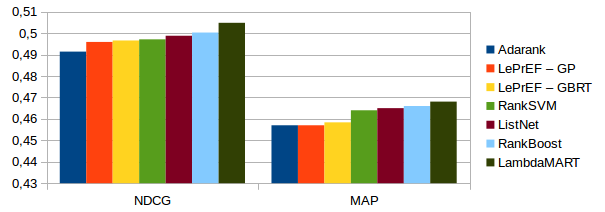
\includegraphics[width=10cm, height=5cm]{im_baseline.png}
\caption{Mean NDCG and MAP results obtained by LePrEF GBRT and other state-of-the-art methods.}
\label{fig:baseline}
\end{center}
\end{figure}


\begin{figure}[h!]
\begin{center}
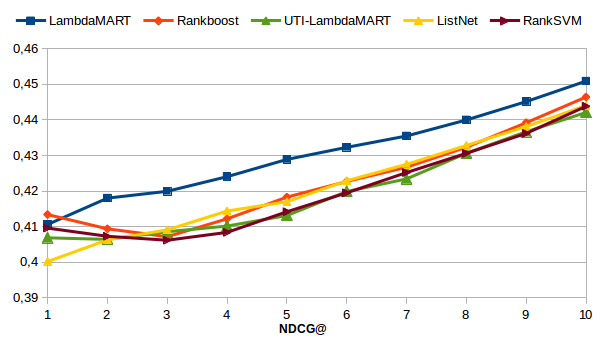
\includegraphics[width=10cm, height=5cm]{im_ndcg_baseline.png}
\caption{Comparison Results with NDCG@1~10 on MQ2007}
\label{fig:ncdg10}
\end{center}
\end{figure}


Other important result is about compression. As explained before, the LePrEF works with features by document-term, so the dataset is bigger than the usual dataset only by query-document. In this case, compression is essential to reduced the inverted list. As can be seen in \ref{fig:crq}, there is indeed a tradeoff between quality and compression rate as the number of decimal point values is reduced. Results with $d=1$ presents a minimal quality variation and a high compression rate. In our experiments the invert list without compression presents 235.244 different UTI's values and 213.140 unique values. In the other hand, with compression, we find only 47 distinct UTI's values and 2 unique values. 

\begin{figure}[h!]
\begin{center}
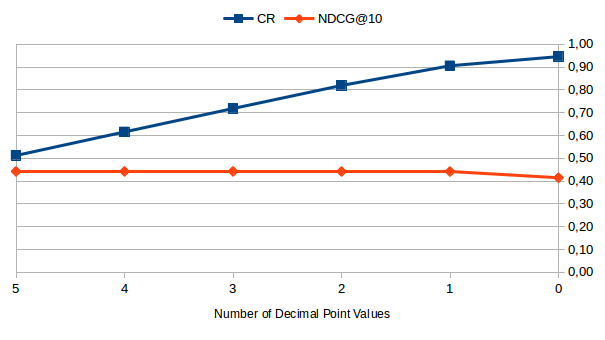
\includegraphics[width=10cm, height=5cm]{im_cr_ndcg_lambda.png}
\caption{Compression Rate (CR) x NDCG@10}
\label{fig:crq}
\end{center}
\end{figure}

\begin{figure*}[h!]
\centering
	\subfigure[UTI without compression. 235.234 distinct values. 213.140 unique values]{%
	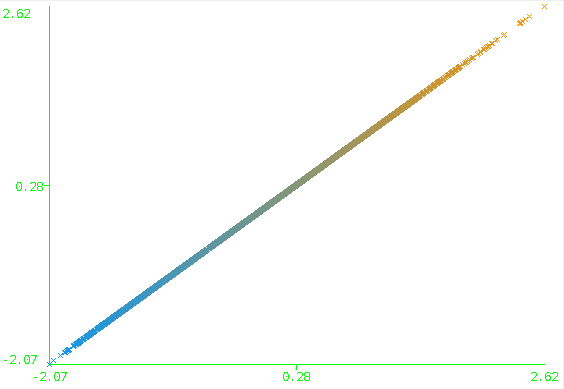
\includegraphics[width=0.4\textwidth]{im_distribuicao_uti_lambda_normal.png}
	\label{fig:dln}}%
	\subfigure[UTI with compression. 47 distinct values; 2 unique values;]{%
	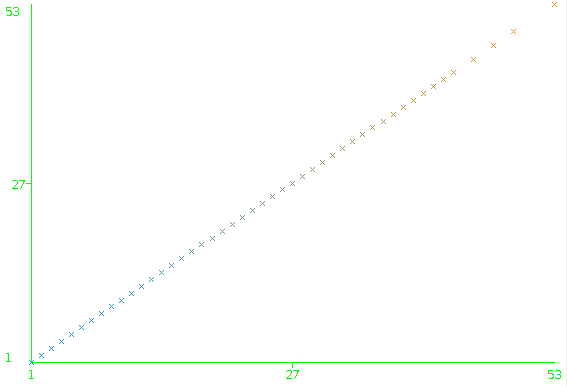
\includegraphics[width=0.4\textwidth]{im_distribuicao_uti_lambda_1casa.png}
	\label{fig:dlc}}
	% 
	\caption{Distribution of 272.140 UTI values for 5 folds without compression (a) and with compression (b).}
	\label{fig:compareData}
\end{figure*}


%Figure~\ref{fig:lfr} shows that LePrEF is superior than BM25, as base ranker. The three top ranker baselines, Rankboost~\cite{freund2003efficient}, CA and LambdaMark, performer better when using the first ranking achieved by LePrEF. This results is interesting to show how we can employ LePrEF in practical web search and the potential benefit that can be achieved by MOL.

%\begin{figure}
%\begin{center}
%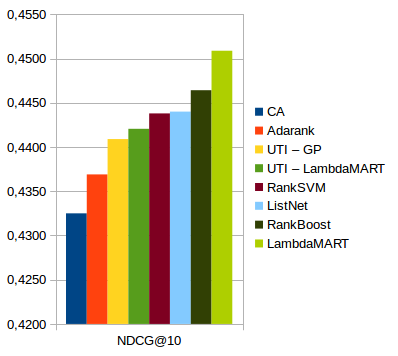
\includegraphics[width=7cm, height=7cm]{im_baselineLePrEF.png}
%\caption{NDCG@10 result obtained by LambdaMART and CA when performed using BM25 and LePrEF as %first ranking.}
%\label{fig:lfr}
%\end{center}
%\end{figure}

%% References
%%
%% Following citation commands can be used in the body text:
%% Usage of \cite is as follows:
%%   \cite{key}         ==>>  [#]
%%   \cite[chap. 2]{key} ==>> [#, chap. 2]
%%

%% References with bibTeX database:

\section{Conclusion}
The experimental results presented in this work indicate that LePrEF GBRT achieve better quality results when compared with LePrEF GP and others implementations, like RanKSVM and AdaRank, despite of use a reduced number of features. 

\label{conclusion}


\bibliographystyle{elsarticle-num}
% \bibliographystyle{elsarticle-harv}
% \bibliographystyle{elsarticle-num-names}
% \bibliographystyle{model1a-num-names}
% \bibliographystyle{model1b-num-names}
% \bibliographystyle{model1c-num-names}
% \bibliographystyle{model1-num-names}
% \bibliographystyle{model2-names}
% \bibliographystyle{model3a-num-names}
% \bibliographystyle{model3-num-names}
% \bibliographystyle{model4-names}
% \bibliographystyle{model5-names}
% \bibliographystyle{model6-num-names}

\bibliography{sample}


\end{document}

%%
%% End of file `elsarticle-template-num.tex'.
